\chapter{Implementierung}
    Hier ein neues Kapitel
    Viele Zitate: \cite{patterson} \cite{krizhevsky} \cite{matlab} \cite{pitts} \cite{lawrence} \cite{miesbach}
    \section{Architektur}
        Eine Section
        \subsection{Subsection}
        
        
Hier ist ein Bild:        
            \begin{figure}[h]
                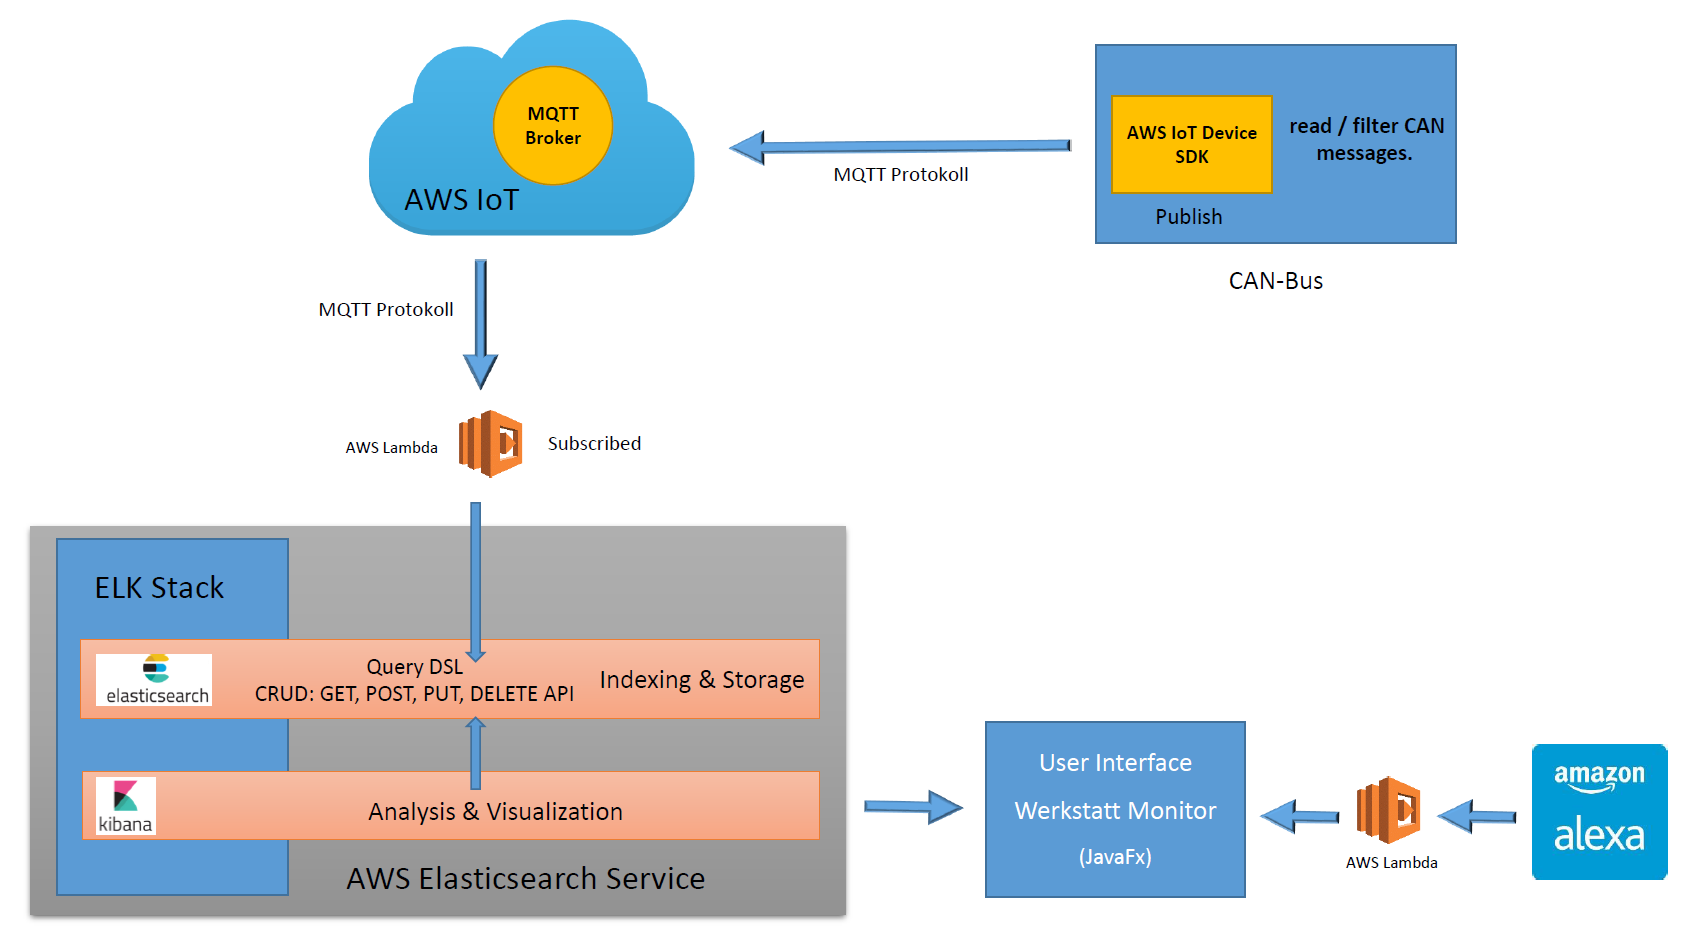
\includegraphics[scale=0.2]{Abbildungen/Kapitel4/Big-architecture.png}
                \centering
                \caption{Affe Bild}
                \label{Abb:Affe}   
            \end{figure}  
            
Hier ist eine Tabelle: text text text text text text text text text text text text text text text text text text text text text text text text text text text text text text text text text text text text text text text text text text text text text text text text text text text text text text text text text text text text text text text text text text text text text text text text text text text text text text text text text text text text text text text text text text text text text text text text text text text text text text text text text text text text text text text text text text text text text text text text text.           
            
             \begin{table}[h]
                \begin{tabular}{ccc}
                      \hline
                      Spalte1 & Spalte2 & Spalte3\\                      
                      \hline
                      1 & 2 & 3\\
                      \hline
                \end{tabular}
                \centering
                \caption{Quadratewurzel Skalierung}
                \label{Tab:Quadratewurzel Skalierung}
            \end{table}
            
Hier eine neue Tabelle: text text text text text text text text text text text text text text text text text text text text text text text text text text text text text text text text text text text text text text text text text text text text text text text text text text text text text text text text text text text text text text text text text text text text text text text text text text text text text text text text text text text text text text text text text text text text text text text text text text text text text text text text text text text text text text text text text text text text text text text text text.   
            
            \begin{table}[h]
                \begin{tabular}{cccc}
                      \hline
                      Spalte1 & Spalte2 & Spalte3 & jbjvh\\                      
                      \hline
                      1 & 2 & 3 & 4\\
                      \hline
                \end{tabular}
                \centering
                \caption{Logaritmische Skalierung}
                \label{Tab:Logaritmische Skalierung}
            \end{table}
 
        
        
    \section{Realisierungsspezifishe Probleme}
        Eine Subsection
	\section{Testkonzept und Testergebnisse}
        Eine Subsection
	\section{interessante Systemteile und Kode}
        Eine Subsection
  